\section{Results}
\label{sec:results}

% FINAL NUMERIC SOURCES (validated 2026-08-23; 17 subjects, seed 42):
% Table 1:
% results/final_paper_experiment/20260823_101436/tables/paper_main_results.csv
% Separate persistence check:
% results/final_paper_experiment/20260823_101436/tables/paper_persistence_result.csv
% Audit/detail files (not the values to transcribe into the main paper table):
% results/final_paper_experiment/20260823_101436/tables/loso_fold_metrics.csv
% results/final_paper_experiment/20260823_101436/tables/persistence_fold_metrics.csv
% results/final_paper_experiment/20260823_101436/tables/cohort_window_counts.csv
% Do not use results/paper/table1_primary_loso_results_15_subject_snapshot.csv;
% that file is the obsolete preliminary 15-subject snapshot.

\begin{table}[t]
	\caption{Leave-one-subject-out results for binary engagement inference, averaged over the 17 held-out participants.
		SD is the standard deviation across participants and $\Delta$ is the improvement in accuracy over the majority baseline, paired within folds.
		Balanced accuracy is relative to 0.500 by construction.
		Accuracy uses all 17 folds.
		The remaining metrics use the 16 folds whose test participant is not single-class.
		M-F1 is macro-F1 and AUC is ROC-AUC\@.
		Best predictive score and paired improvement in bold.}
	\label{tab:main}
	\setlength{\tabcolsep}{3.2pt}
	\footnotesize
	\begin{tabular}{lcccccc}
		\toprule
		                    & Acc.          & SD   & $\Delta$         & Bal.\ acc.    & M-F1          & AUC           \\
		\midrule
		Majority baseline   & .524          & .346 & ---              & .500          & .326          & .500          \\
		\midrule
		\multicolumn{7}{l}{\emph{Raw signals} (600-d)}                                                                \\
		\quad Random forest & .527          & .147 & $+.003$          & .529          & .460          & .546          \\
		\quad MLP           & \textbf{.538} & .113 & $\mathbf{+.014}$ & \textbf{.536} & \textbf{.468} & \textbf{.551} \\
		\midrule
		\multicolumn{7}{l}{\emph{Handcrafted features} (58--60-d)}                                                    \\
		\quad Random forest & .528          & .230 & $+.005$          & .508          & .418          & .527          \\
		\quad MLP           & .531          & .145 & $+.008$          & .521          & .451          & .535          \\
		\midrule
		\multicolumn{7}{l}{\emph{GazeMAE embeddings} (256-d)}                                                         \\
		\quad Random forest & .535          & .155 & $+.012$          & .509          & .441          & .513          \\
		\quad MLP           & .520          & .107 & $-.004$          & .493          & .435          & .494          \\
		\midrule
		\multicolumn{7}{l}{\emph{MOMENT embeddings} (1{,}024-d)}                                                      \\
		\quad Random forest & .521          & .286 & $-.002$          & .501          & .380          & .504          \\
		\quad MLP           & .507          & .274 & $-.017$          & .497          & .362          & .504          \\
		\bottomrule
	\end{tabular}
\end{table}

Table~\ref{tab:main} reports the main comparison.
Every representation--model combination sits close to the majority baseline.
The highest observed result is the raw signal with the MLP, at 0.538 accuracy, 0.014 above the paired baseline, and it is also highest on balanced accuracy (0.536), macro-F1 (0.468) and ROC-AUC (0.551).
Handcrafted features give the next-highest balanced accuracy, macro-F1 and ROC-AUC, and improve on the baseline accuracy with both classifiers.
GazeMAE reaches 0.535 accuracy with the random forest and falls to 0.520, below the baseline, with the MLP\@.
MOMENT falls below the baseline accuracy with both classifiers, while its balanced accuracy and ROC-AUC remain close to chance.

Raw signals give the highest value on every metric.
Handcrafted features rank second on the three secondary discrimination metrics, while GazeMAE has the second-highest accuracy.
The paired accuracy changes range from $-0.017$ to $+0.014$, much less than the spread across held-out participants, whose accuracy standard deviations range from 0.11 to 0.29.
The MLP improves raw and handcrafted inputs but lowers both embedding results.
A flexible head may help when a representation already carries useful signal.
The effect is small, so this interpretation remains tentative.

\begin{figure*}[t]
	\centering
	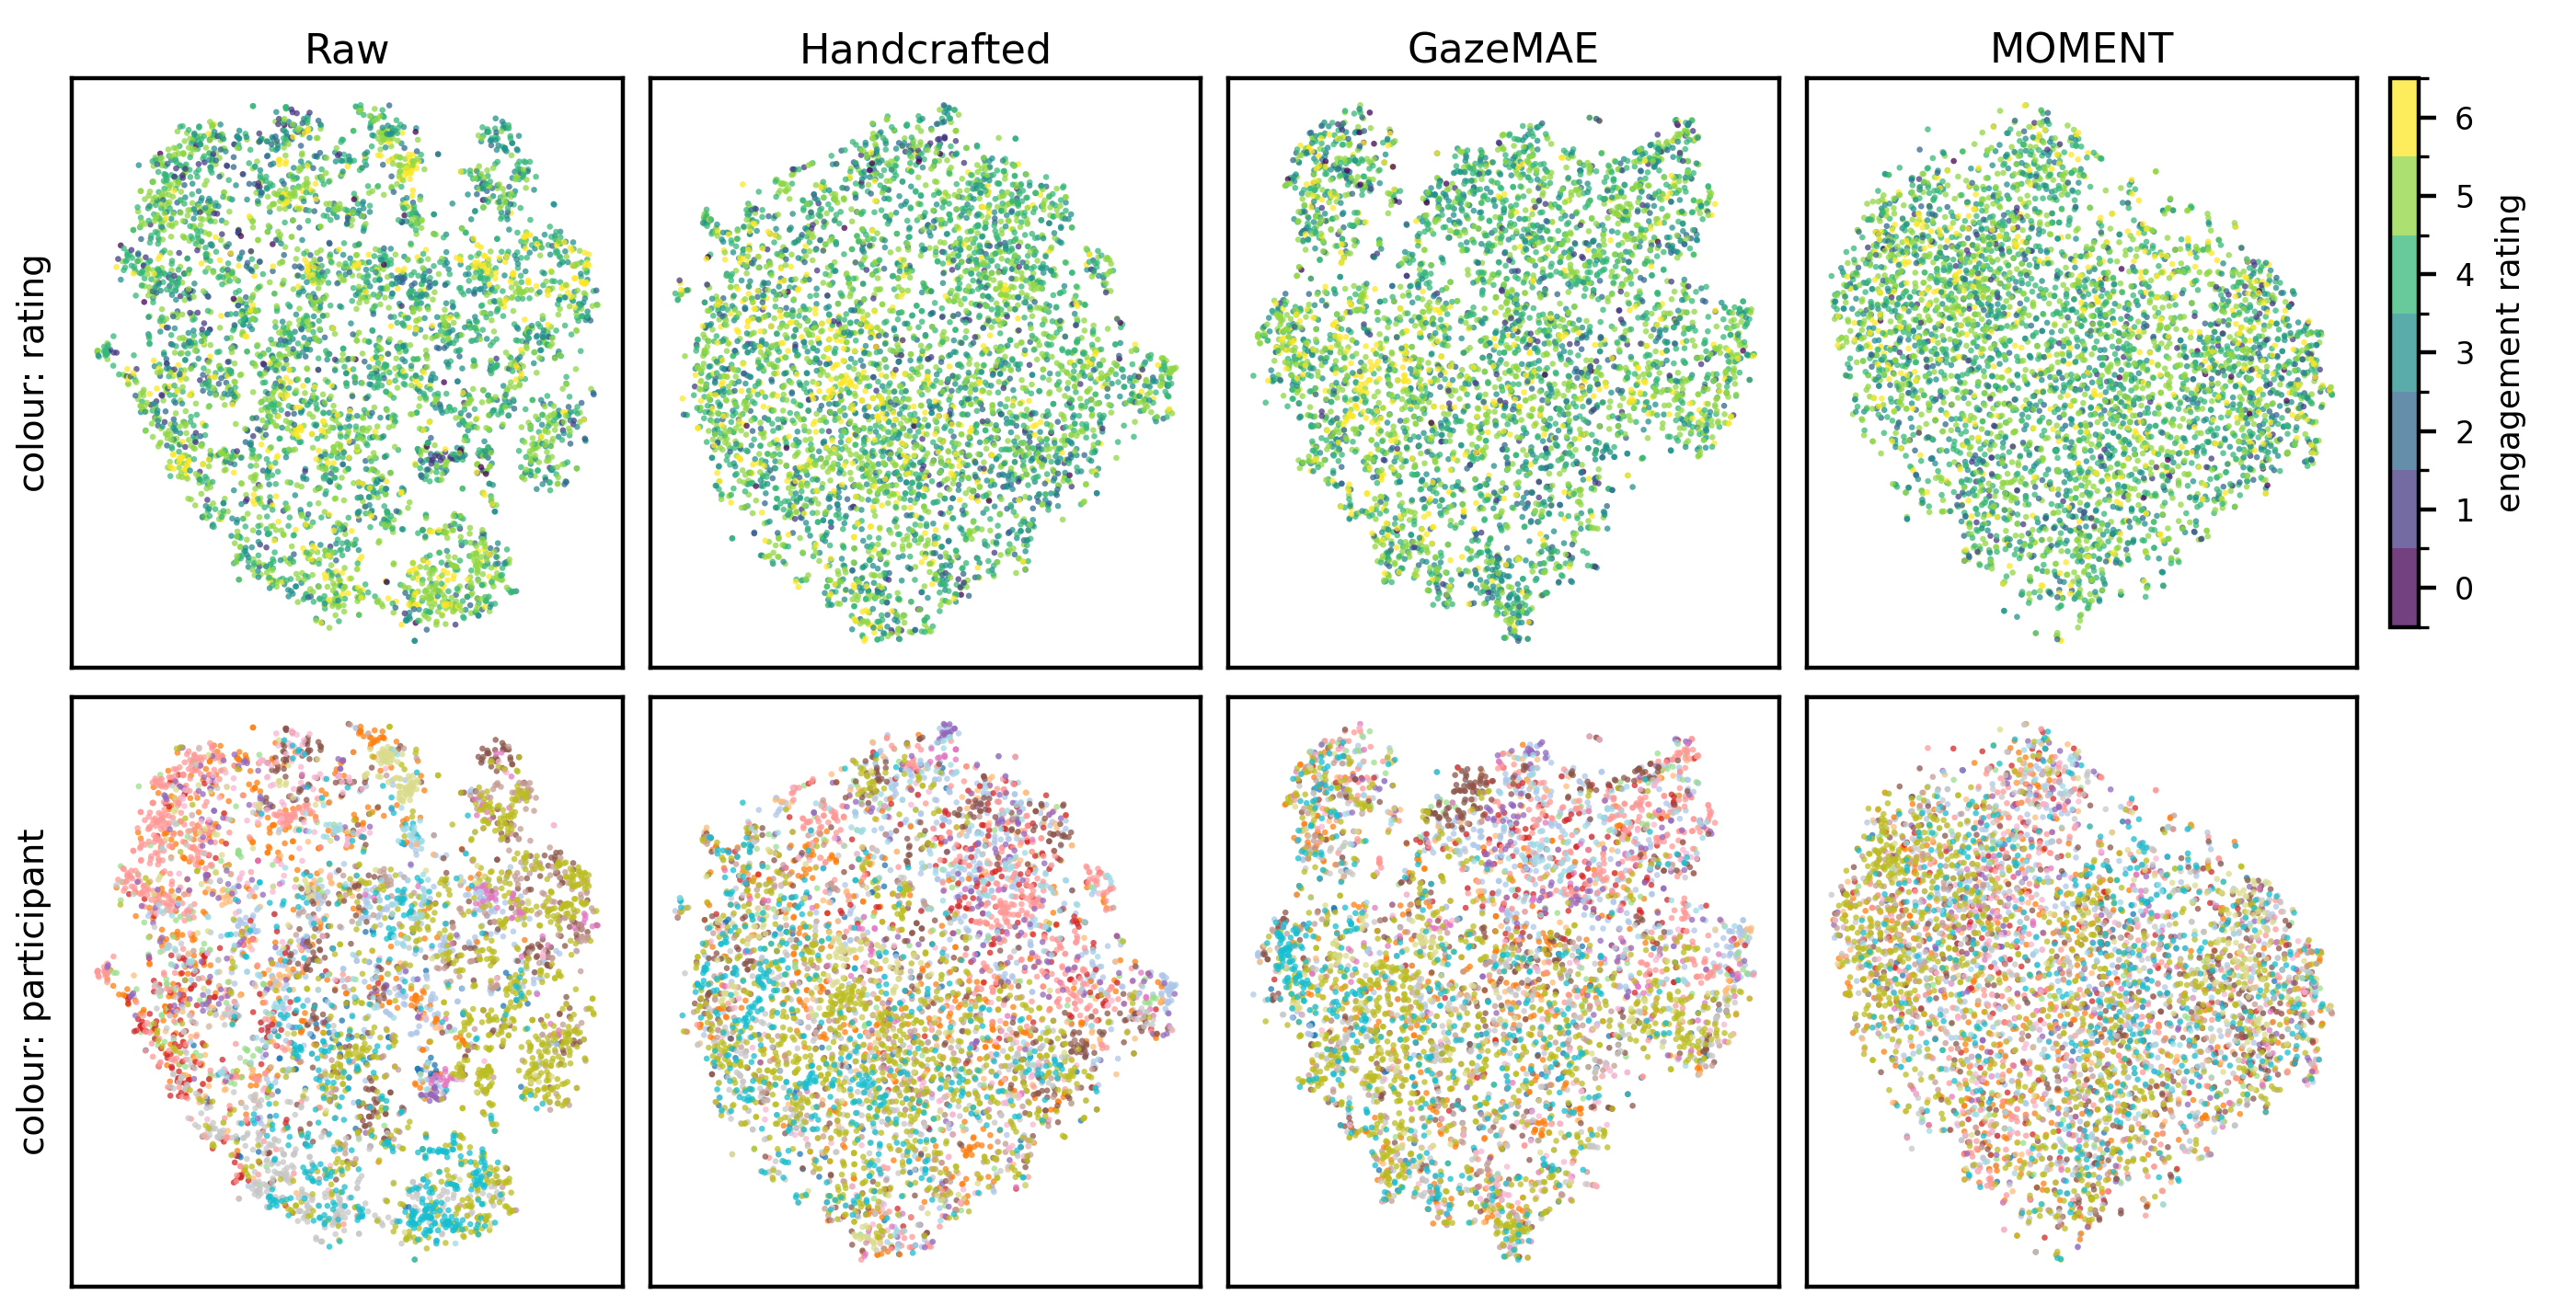
\includegraphics[width=\textwidth]{figures/fig2_tsne.png}
	\Description{Eight scatter plots arranged in two rows of four, showing t-SNE projections of the four representations coloured by engagement rating and by participant.}
	\caption{t-SNE projections of the four representations over a common sample of 5{,}000 windows, coloured by engagement rating (top) and by participant (bottom).
		Participant colours form visible patches in the raw projection and mix almost uniformly in the MOMENT projection, while no projection shows regions that follow the engagement rating.}
	\label{fig:tsne}
\end{figure*}

Figure~\ref{fig:tsne} shows the same difficulty geometrically.
In the t-SNE projections, none of the four representations arranges windows by engagement rating, and the colours are as mixed in the learned embeddings as in the raw signal.
Colouring the identical projections by participant is more informative.
Raw signals form clear participant-dominated patches, handcrafted features and GazeMAE group more weakly, and the MOMENT projection is close to uniform.
The clearest visible structure is therefore person-specific, and the weaker grouping in the frozen embeddings may reflect smoothing by the encoders.
Because the projections are exploratory, this interpretation and its link to Table~\ref{tab:main} remain conjectures.

As a check on the label series, a one-step persistence predictor is evaluated over 1{,}434 temporal blocks.
Participant-averaged accuracy reaches 0.999, while balanced accuracy reaches 0.960 and macro-F1 reaches 0.965 over the 13 participants with two-class test blocks.
Each questionnaire answer is broadcast unchanged to every window of the preceding 15-minute interval (Section~\ref{sec:method}), so most consecutive window pairs share a label by construction.
Because the predictor uses observed labels within participants, its result cannot be compared directly with the unseen-participant results above.
